


\chapter{Statistical Decision Theory}
\label{sec:desicion_theory}

This section follows the spirit of Section~7 in \cite{hastie_elements_2003}, up to some changes in notation.

In Section~\ref{sec:learning}, we gave an intuitive argument for which without some inductive bias, learning will return models with poor performance on new data.
In this section we learn how to quantify the performance of a model. In particular, when given new data. This allows us to select among competing candidate models. It will also allow us to choose the value of the regularization parameter of each method.

Figure~\ref{fig:bias_variance} demonstrate the prediction error (red curve) of some model as the model complexity increases. As can be seen, the prediction error decreases as the model becomes more complex, but saturates at some point. 
This is because the reduction in the bias is smaller than the increase in variance of learning very complex models.
This is the celebrated bias-variance tradeoff.\marginnote{Bias Variance Tradeoff}

Once we are able to estimate the prediction error from our data, we will seek for a model which minimizes this error.

\begin{figure}[h]
        \centering
        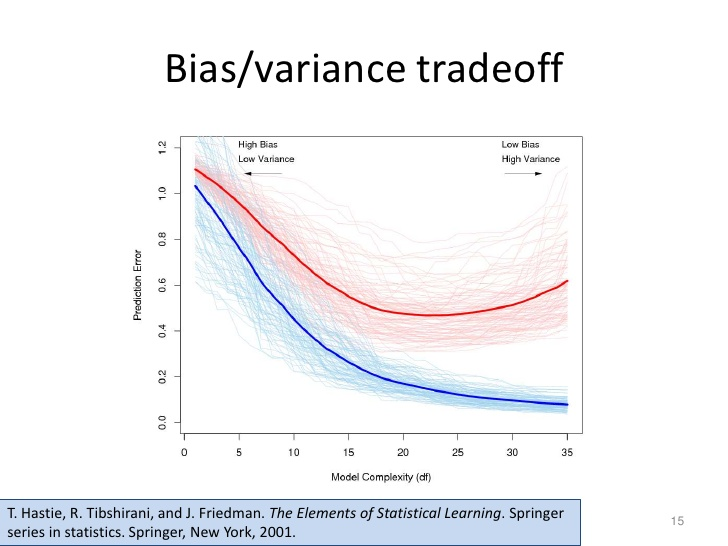
\includegraphics[width=1\textwidth]{art/support-vector-machine-15-728}
        \caption{Overfitting: 
        Prediction error on new data (red curve) versus the empirical prediction error (light blue).
        The empirical prediction error will always decrease as more complicated models are fit (moving right).
        The prediction error on new data, however, will not always decrease and will typically show a local minima.
        \label{fig:bias_variance}}
\end{figure}

Before we proceed, we now need to distinguish between several types of prediction errors.
The population \emph{risk} of a model parametrized by $\theta$, was previously defined as the average loss over all possible data instances, and denoted by $\risk(\theta)$ (\S \ref{sec:m_estimation}).
The empirical risk was defined as the average loss over the observed data points, and denoted by $\riskn(\theta)$.
We now update these definitions to deal with the the $\hyp(x)$ notation of the previous section.
\begin{align}
	\test :=& \expectg{Y,X}{\loss(Y,\hyp(X))}, \label{eq:test_error} \\
	\train :=& \expectn{\loss(y,\hyp(x))} = \frac{1}{n} \sum_i \loss(y_i,\hyp(x_i)),  \label{eq:training_error} \\
	\insample :=& \frac{1}{n} \sum_i \expectg{Y}{\loss(Y,\hyp(x_i))}, \label{eq:in_sample} \\
	\EPE :=& \expectg{\estim{\hyp}_n}{
		\expectg{Y,X}{\loss(Y,\estim{\hyp}_n(X))|\estim{\hyp}_n}
	}.\label{eq:epe}
\end{align}

Eq.(\ref{eq:test_error}) is merely a reformulation of $\risk(\theta)$ from Section~\ref{sec:m_estimation}.
It captures the expected loss, a given predictor, $\hyp(X)$, will incur on average when given new $X$'s and $Y$'s.
This will be the magnitude which will tell us which models perform well, and which do not.
It is known as the \emph{test error} or also as \emph{prediction error}.\marginnote{Test Error}

Eq.(\ref{eq:training_error}) is the reformulation of empirical risk, $\riskn(\theta)$, we have been optimizing in Section~\ref{sec:learning}.
We referred to it as the \emph{empirical risk}, but it is also known as the \emph{train error}.
\marginnote{Train Error}

Eq.(\ref{eq:in_sample}) is the average risk at the observed $x$'s, when given new $Y$'s \footnote{This magnitude should not be unfamiliar: e.g., inference in ANOVA is performed conditional on the $x$'s, which typically stem from a designed experiment.}.
This is the \emph{in sample error}.
\marginnote{In Sample Error}

Eq.(\ref{eq:epe}) is called the \emph{expected prediction error}, i.e., the expected loss when $\hyp$ is also re-learned. 
Put differently: How much would we err when:(1) we are given $n$ new examples $\sample_1$; (2) re-learn $\estim{\hyp}_n$ on $\sample_1$; (3) compute the risk of $\estim{\hyp}_n$ (in the population, not in $\sample_1$.
We emphasize this by writing $\estim{\hyp}_n$ instead of $\hyp$.
$\EPE$ is thus not a property of a particular predictor $\hyp$, but rather of a whole learning algorithm on random samples of size $n$.
It could have also been written as $\risk(algorithm)$, although I have not seen this notation in use.
\marginnote{Expected Prediction Error}


We would like to compare the performance of models based on $\test$, as this will give us an idea on the quality of the prediction on new data. 
Alas, computing $\test$ requires the distribution of $y$ and $x$, while we only have access to the $n$ observed samples.
Can the empirical risk $\train$ estimate the unknown risk $\test$? 
Figure~\ref{fig:bias_variance} suggests it cannot since $\train$ underestimates $\test$.
Why is this?
At an intuitive level: this is because with ERM we learn the $\hyp$ with smallest error in each sample.
It is thus the same as estimating the expected height in a population, by using the minimum in each sample; we will clearly be underestimating the expectation. Then again, there is the hope that we may take this minimum and debias it. 
This is the goal in the next sections.

Before proceeding, we distinguish between two similar tasks: 
\begin{description}
\item[Model Selection] This is the task of selecting between several candidate models.
\item[Model Assessment] This is the task of assessing the prediction error (i.e., the expected loss, the risk) of a given model.
\end{description}



\section{Train, Validate, Test}
\label{sec:train_test}
If data is abundant, a trivial, assumption free way to estimate $\test$\footnote{Think: why $\test$ is being estimated, and not $\EPE$ nor $\insample$?}, is to split the data into $3$ sets.
A \emph{training set}, used to learn several competing models.
A \emph{validation set}, used check the performance of the learned models and choose the best performer using some comparison measure. 
A \emph{test set}, used to estimate the risk, as the empirical risk $\train$ will be unbiased to the population risk $\test$.

If there is not enough data for this scheme, keep reading...


\section{Unbiased Estimators of the Risk}
\label{sec:risk_estimation}
Under appropriate assumptions, the bias in $\train$ when estimating $\insample$\footnote{In this case, note that it is $\insample$ being estimated, and not $\test$ nor $\EPE$.} can be computed analytically, and accounted for.
The bias $\insample-\train$ is called the \emph{optimism} of the algorithm.\marginnote{Optimism}
Akaike's Information Criterion (AIC), 
the finite sample Corrected AIC (AICc), 
Mallow's Cp (Cp), 
the Bayesian Information Criterion (BIC, aka SBC, aka SBIC), 
the Minimum Description Description Length (MDL), 
Vapnic's Structural Risk Minimization (SRM), 
the Deviance Information Criterion (DIC), 
and the Hannan-Quinn Information Criterion (HQC), 
all try to estimate $\insample$ by correcting for the optimism under different assumptions.\marginnote{Cp, AIC, BIC, MDL, SRM}

The differences, pros, and cons, of each will not be discussed herein. Just remember what they mean when you see them in your favourite software (R!).
They all have in common that you will want the model with the smallest criterion.
But be careful- as they are used for model selection, they are indifferent to scaling, and thus should be not interpreted as the expected prediction error.

\begin{remark}
Not all model selection criteria estimate $\insample$. The Focused Information Criterion (FIC), for example, does not.
\end{remark}





\paragraph{Further Reading}
For a brief review of AIC, BIC, MDL and SRM see Chapter 7 in \citep{hastie_elements_2003}. 
For a more rigorous derivation, see \cite{claeskens_model_2008}.





\section{Jackknifing}
\label{sec:jackknife}

If concerned with over fitting, here is a simple algorithm to estimate the prediction error:

\begin{algorithm}[H]
\caption{Jackknife}
\begin{algorithmic}
\For {$i \in 1,\dots,n$}
    \State $\estim{\hyp}^{(i)} \gets$ the learned model with all but the $i$'th observation.
    \State $\loss^{(i)} \gets$ the loss of $\estim{\hyp}^{(i)}$ on the $i$'th observation.
\EndFor
\State \Return the average loss over $\loss^{(i)}$.
\end{algorithmic}
\end{algorithm}

This process is called the \emph{Jackknife}, or \emph{Leave-One-Out--Cross-Validation}. 
This algorithm return an estimator of $\EPE$.
This might be quite surprising: every split uses almost an identical sample, so why would it not estimate $\test$? See Section 7.12 in \cite{hastie_elements_2003} for details..

But wait! We might be able to stabilize the variability of the estimated error in every split, if instead of leaving only a single observation aside, we leave some more. This lead to way to \emph{K-Fold Cross Validation} in the next section.


\section{Cross Validation}
\label{sec:cv}

\begin{algorithm}[H]
\caption{Cross Validation}
\begin{algorithmic}
\State Split the data into $\folds$ parts (``folds'').
\For {$\fold \in 1,\dots,\folds$}
    \State $\estim{\hyp}^{(k)} \gets$ the learned model with all \emph{except} the observations in the $\fold$'th fold.
    \State $\loss^{(\fold)} \gets$ the loss average of $\estim{\hyp}^{(\fold)}$ on the observations in the $\fold$'th fold.
\EndFor
\State \Return the average over $\loss^{(\fold)}$ .
\end{algorithmic}
\end{algorithm}

This simple algorithm estimates $\EPE$ without any assumption on the data generating process, and less data than would be required for a ``train-validate-test'' scheme.
Well, as it actually serves for model selection, it should be seen as a ``train-validate'' scheme, without the ``test'' part. It is thus \emph{not} an unbiased estimate of $\EPE$. See Section 7.12 in \cite{hastie_elements_2003} for details.

But wait again! 
The Cross Validation scheme resamples the data \emph{without replacement} to estimate $\EPE$. Could we have sampled it \emph{with} replacement? Yes. This is the idea underlying the \emph{Bootstrapping} scheme.


\section{Bootstrapping}
\label{sec:bootstrap}

Here is the simplest version of Bootstrap validation:

\begin{algorithm}[H]
\caption{Bootstrap}
\begin{algorithmic}
\For {$\bootstrap \in 1,\dots,\bootstraps$}
	\State $\sample^\bootstrap \gets$ $n$ randomly selected observations, with replacement, from the original data.
    \State $\estim{\hyp}^{\bootstrap} \gets$ the model learned with  $\sample^\bootstrap$.
    \State $\loss^{\bootstrap} \gets$ the average loss of $\estim{\hyp}^{\bootstrap}$ on the observations in the \emph{original} data.
\EndFor
\State \Return the over of $\loss^{\bootstrap}$ .
\end{algorithmic}
\end{algorithm}

This algorithm is not a good estimator of $\EPE$ as observations play a role both in learning and in validating. 
Several corrections are available. For details see Section 7.11 in \cite{hastie_elements_2003}.

The Bootstrap is a very general scheme, which can be used not only for model validation, but for assessing many of its statistical properties. It is possibly best known when used for hypothesis testing. 
For more on the Bootstrap, see \cite{efron_introduction_1994}.

